\documentclass{beamer}

\usepackage{graphicx}
\usepackage{listings}

\usepackage{natbib}

\usetheme{Berkeley}

\title[About Lex]{About Lex/Flex}
\subtitle{And little bit on Yacc/Bison}
\author{Vikrant Gajria\inst{1}}
\institute{
    \inst{1} BE Computer Engineering,
    DJSCE
}
% \logo{
\includegraphics[height=1.2cm,width=1.2cm]{./imgs/logo.png}}

\date{24 March 2021}

% -----

\begin{document}

% -----
\begin{frame}
    \maketitle
\end{frame}

% ----------
\section{Lexical Analysis}

% -----
\begin{frame}
    \frametitle{Lexical Analysis}

    \begin{figure}
        \centering
        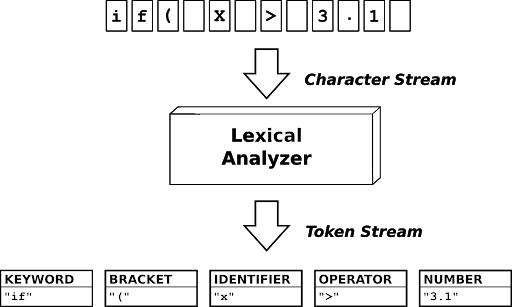
\includegraphics[width=\textwidth]{./imgs/lexer.png}
        \caption{Lexer operation}
        \label{fig:lexer}
    \end{figure}
\end{frame}

% -----
\begin{frame}
    \frametitle{Lexical Analysis}

    \[ <token, value> \]

    \begin{itemize}
        \item token = unique integer value, e.g. ID = 1, INT = 2
        \item value (optional) = data related to token, e.g. ``x'', 5
    \end{itemize}

    Hence, we have $<ID, ``x">$, $<INT, 5>$
\end{frame}

% -----
\begin{frame}
    \frametitle{Lexical Analysis}

    \begin{figure}
        \centering
        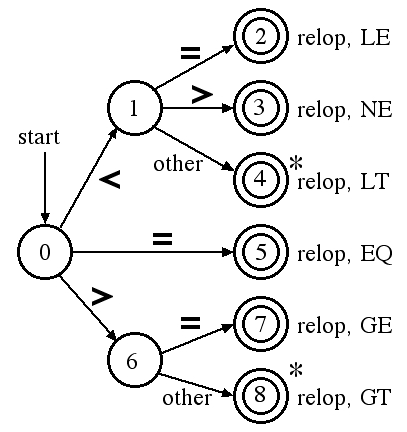
\includegraphics[height=4cm]{./imgs/dfa.jpg}
        \caption{Lexical Analysis as a DFA}
        \label{fig:dfa}
    \end{figure}

    \begin{block}{Problem}
        Writing so much logic is very tedious and unmaintainable in code!
    \end{block}
\end{frame}

% ----------
\section{Lex/ Flex}

% -----
\begin{frame}
    \frametitle{Lex/ Flex}

    \begin{itemize}
        \item Computer program that generates lexical analyzers (also known as ``scanners"" or ``lexers'')
        \item Flex (fast lexical analyzer generator) is a free and open-source software alternative to lex
    \end{itemize}

    It is not a framework or a library, it writes the code for you
\end{frame}

% -----
\begin{frame}
    \frametitle{Why Lex}

    \begin{itemize}
        \item Write rules, not code
        \item Regular Expression ``Patterns'' for DFA building
        \item Streaming lexer, does not load entire files all at once
        \item Hence, it is extremely fast
        \item Written for C orignally but can be used for C++
        \item Reimplemented for other languages like Rust, Go, Python...
    \end{itemize}
\end{frame}

% ----------
\subsection{Example 1}

% -----
\begin{frame}[fragile]
    \frametitle{Generating code}
    
    \begin{verbatim}
%%

[0-9]           printf("Digit: %s \n", yytext);
\n              printf("New line \n");
.               printf("Any: %s \n", yytext);
    \end{verbatim}
    
    These 4 lines generate 1734 lines of C code!
    
    \begin{block}{\%\% Sections}
        The \%\% is important because it marks the start of Rules sections
    \end{block}
\end{frame}

% -----
\begin{frame}
    \frametitle{Example 1}
    
    \begin{figure}
        \centering
        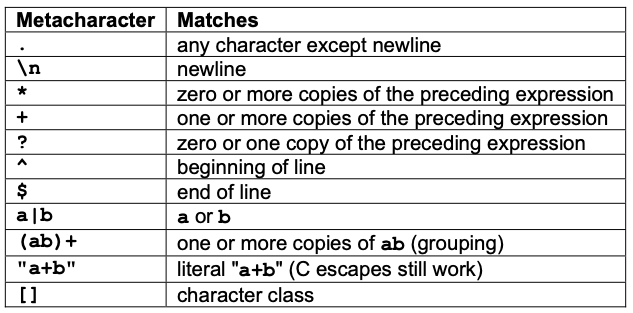
\includegraphics[height=4cm]{imgs/regex.png}
        \caption{Regex pattern primitives}
        \label{fig:regex}
    \end{figure}
    
    \begin{alertblock}{yytext}
        yytext is a global variable that stores the text of the lexeme matched by regex.
    \end{alertblock}
\end{frame}

% -----
\begin{frame}[fragile]
    \frametitle{Using flex}
    
    Generate code using:
    \begin{verbatim}
        flex <filename>
        gcc -lfl lex.yy.c -o <outputname>
    \end{verbatim}
    
    Run interactive mode:
    \begin{verbatim}
        ./<outputname>
    \end{verbatim}
    
    Pass in a file's text:
    \begin{verbatim}
        cat <file> | ./<outputname>
    \end{verbatim}
\end{frame}

% ----------
\subsection{Example 2}

% -----
\begin{frame}[fragile]
    \frametitle{Example 2}
    
    \begin{verbatim}
DIGIT    [0-9]
ID       [a-zA-Z][a-zA-Z0-9]*

%%

[\t ]           { /* Perform no action */ }
{DIGIT}+        printf("Digit: %s \n", yytext);
{ID}            printf("Identifier: %s \n", yytext);
\n              printf("New line \n");
    \end{verbatim}
    
    \begin{block}{\%\% Sections}
        The section above \%\% is Declarations section with C code, declarations (DIGIT, ID), and other configurations.
    \end{block}
\end{frame}

% ----------
\subsection{Example 3}

% -----
\begin{frame}[fragile]
    \frametitle{Example 3}
    
    \begin{lstlisting}[basicstyle=\tiny, language=c]
... declarations

%%
... rules

%%

int main(argc, argv)
int argc;
char **argv;
{
    ++argv, --argc;
    if ( argc > 0 )
            yyin = fopen( argv[0], "r" );
    else
            yyin = stdin;

    yylex();
}
    \end{lstlisting}
    
    \begin{block}{\%\% Sections}
        An optional user code section can be added after the rules.
        This section is copied verbatim, i.e. directly into the generated code.
    \end{block}
\end{frame}

\begin{frame}
    \frametitle{Example 3}
    
    \begin{alertblock}{yyin}
        File to be processed. Set it to a readable file pointer.
        Default is stdin i.e. command line input.
    \end{alertblock}
    
    \begin{alertblock}{yylex}
        Continuously lexically analyse a file. If you return something,
        it will pause execution and start again if you call it again.
        You can change the return type by modifying YYDECL macro (advanced).
    \end{alertblock}
\end{frame}

% ----------
\section{Summary}

% ----------
\subsection{Code structure}

% -----
\begin{frame}[fragile]
    \frametitle{Syntax}
    
    \begin{lstlisting}[basicstyle=\tiny]
[
%{
... user code for header files and other config
%}
]

... declarations, if any

%%
... rules in tabular form, regex and action

[
%%
... user code for anything after the rules, like main
]
    \end{lstlisting}
    
    Where $[ block ]$ means optional
    
    \begin{alertblock}{Standard structure}
        This structure is used in all Lex implementations.
        Yacc and its implementations also uses same structure!
    \end{alertblock}
\end{frame}

% ----------
\subsection{Variables}

% -----
\begin{frame}
    \frametitle{yyVariables}

    \begin{figure}
        \centering
        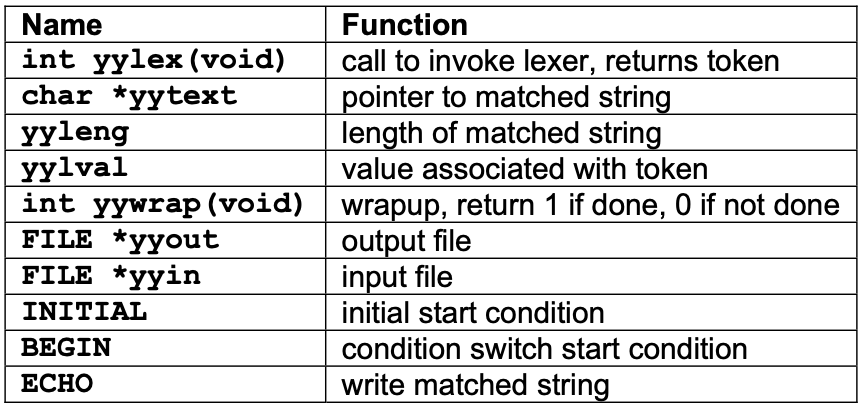
\includegraphics[height=5cm]{imgs/vars.png}
        \caption{Predefined global variables}
        \label{fig:variables}
    \end{figure}
\end{frame}

% ----------
\section{More examples}

% ----------
\subsection{Assembly-like language}

\begin{frame}[fragile]
    \frametitle{Example 4}
    
    \textbf{Assembly-like calculator}
    
    \begin{lstlisting}[basicstyle=\small]
ADD 5;
PRINT;

* 4;
PRINT;
/ -2;
ADD 7;
PRINT;

sub 13;
print;

clear;
print;
EXIT;
    \end{lstlisting}
\end{frame}

% ----------
\subsection{Yacc/ Bison}

% ----------
\subsubsection{Parsing}

\begin{frame}
    \frametitle{Yacc - Parser Generator}

    \begin{figure}
        \centering
        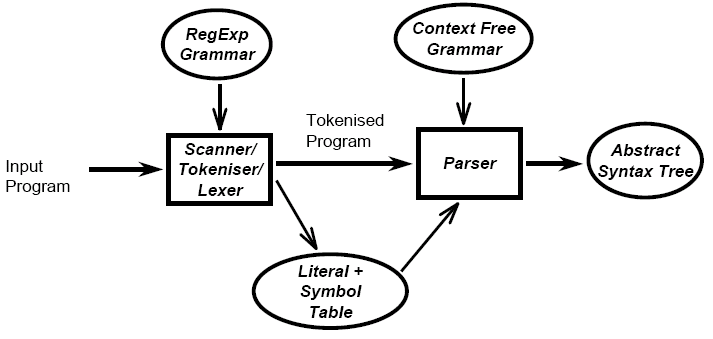
\includegraphics[height=5cm]{imgs/parsingpipeline.png}
        \caption{Lexer to Parser pipeline}
        \label{fig:parser}
    \end{figure}
\end{frame}

% ----------
\subsubsection{Integration}

% -----
\begin{frame}
    \frametitle{Integrating Yacc/Bison with Lex/Flex}

    \begin{figure}
        \centering
        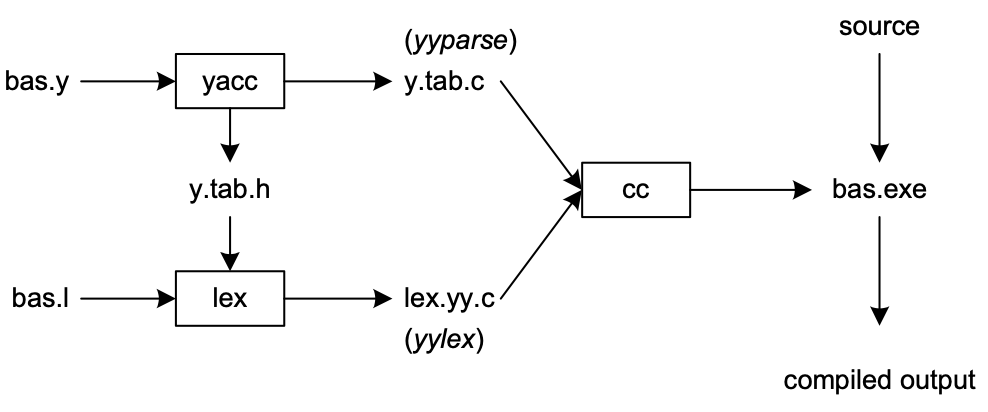
\includegraphics[width=0.75\textwidth]{imgs/yacc.png}
        \caption{Steps to compile Lex and Yacc/ Flex and Bison}
        \label{fig:yacc}
    \end{figure}
    
    \begin{alertblock}{yylval}
        yylval, defined in $.tab.c$, is used to store data related to tokens (value from $<token, value>$).
        It's datatype is defined using YYSTYPE macro and is usually defined using Yacc/ Bison.
    \end{alertblock}
\end{frame}

% -----
\begin{frame}[fragile]
    \frametitle{Example 5}
    
    \textbf{Calculator with infix syntax}
    
    \begin{lstlisting}
    1 + 2
    3.0 / 2
    2 * (3.1427 / 3)
    1.1 + 2 - 3 * 4 / 5.
    \end{lstlisting}
    
    Is based on
    \begin{lstlisting}
    E -> E + E | E - E | T
    T -> T * F | T / F | F
    F -> ( E ) | num | id
    \end{lstlisting}
    
    Code is generated using Yacc/ Bison
\end{frame}

% ----------
\section{D.I.Y.}

% -----
\begin{frame}
    \frametitle{Experiment yourself}
    
    \begin{itemize}
        \item CSV parser using Flex
        \item HTML/ XML parser using Flex
        \item JSON/ YAML/ TOML/ CFG/ INI parser using Flex or Flex+Bison
        \item Assembly-like stack machine using Flex or Flex+Bison
        \item Pascal/ TCL/ C language parser using Flex+Bison
        \item Use C++ and multiple files, explore the option flags
    \end{itemize}
\end{frame}

% ----------
\section{References}

% -----
\begin{frame}
    \nocite{*}
    \bibliographystyle{unsrtnat}
    {\tiny \bibliography{ref.bib} }
\end{frame}

% -----

\end{document}

% -----

